% /**
% * Copyright 2012 Sergio García Mondaray
% *
% * This file is part of GodTIC-Templates (www.godtic.com).
% * 
% * GodTIC-Templates is free software: you can redistribute it and/or modify it
% * under the terms of the GNU General Public License as published by
% * the Free Software Foundation (version 3 of the License).
% * 
% * GodTIC-Templates is distributed in the hope that it will be useful, but
% * WITHOUT ANY WARRANTY; without even the implied warranty 
% * of MERCHANTABILITY or FITNESS FOR A PARTICULAR PURPOSE. 
% * See the GNU General Public License for more details.
% * 
% * You should have received a copy of the GNU General Public License 
% * along with GodTIC-Templates. If not, see http://www.gnu.org/licenses/.
% **/

%%%%%%%%%%%%%%%%%%%%%%%%%%%%%%%%%%%%%%%%%%%%%%%%%%%%%%%%%%%%%%%%%%%%%%
\documentclass[12pt]{beamer}% /**
% * Copyright 2012 Sergio García Mondaray
% *
% * This file is part of GodTIC-Templates (www.godtic.com).
% * 
% * GodTIC-Templates is free software: you can redistribute it and/or modify it
% * under the terms of the GNU General Public License as published by
% * the Free Software Foundation (version 3 of the License).
% * 
% * GodTIC-Templates is distributed in the hope that it will be useful, but
% * WITHOUT ANY WARRANTY; without even the implied warranty 
% * of MERCHANTABILITY or FITNESS FOR A PARTICULAR PURPOSE. 
% * See the GNU General Public License for more details.
% * 
% * You should have received a copy of the GNU General Public License 
% * along with GodTIC-Templates. If not, see http://www.gnu.org/licenses/.
% **/

\usepackage[utf8]{inputenc}
\usepackage[spanish]{babel}

\usetheme{/theme}
\usepackage{thumbpdf}
\usepackage{wasysym}
\usepackage{ucs}
\usepackage{pgf,pgfarrows,pgfnodes,pgfautomata,pgfheaps,pgfshade}
\usepackage{verbatim}
\usepackage{hyperref}
\usepackage{pifont}
\usepackage{color}
\usepackage{wrapfig}
\usepackage{graphicx}
\definecolor{mygreen}{rgb}{0,0.7,0.1}
\definecolor{myorange}{rgb}{1,0.5,0}

\graphicspath{{img/}} 
\DeclareGraphicsExtensions{.pdf,.png,.jpg}
\usepackage{listings}

\usepackage{color}
\definecolor{lightgray}{rgb}{.9,.9,.9}
\definecolor{darkgray}{rgb}{.4,.4,.4}
\definecolor{purple}{rgb}{0.65, 0.12, 0.82}

\lstdefinelanguage{JavaScript}{
  keywords={typeof, new, true, false, catch, function, return, null, catch, switch, var, if, in, while, do, else, case, break},
  keywordstyle=\color{blue}\bfseries,
  ndkeywords={class, export, boolean, throw, implements, import, this},
  ndkeywordstyle=\color{darkgray}\bfseries,
  identifierstyle=\color{black},
  sensitive=false,
  comment=[l]{//},
  morecomment=[s]{/*}{*/},
  commentstyle=\color{purple}\ttfamily,
  stringstyle=\color{red}\ttfamily,
  morestring=[b]',
  morestring=[b]"
}

\lstset{tabsize=4,
  showspaces=false,
  showtabs=false,
  frame=l,
  framerule=1pt,
  aboveskip=0.5cm,
  framextopmargin=3pt,
  framexbottommargin=3pt,
  framexleftmargin=18pt,
  framesep=.4pt,
  rulesep=.4pt,
  stringstyle=\ttfamily,
  showstringspaces = false,
  basicstyle=\footnotesize\ttfamily,
  keywordstyle=\bfseries,
  numbers=left,
  numbersep=6pt,
  numberstyle=\color[cmyk]{0.43, 0.35, 0.35,0.01}\bfseries\scriptsize\ttfamily,
  numberfirstline = true,
  breaklines=true,
  stepnumber=1,
  backgroundcolor=\color{white},
  xleftmargin=18pt,
  framexrightmargin=0pt,
  xrightmargin=0pt,
  language=JavaScript
}
 %%%%%% METADATOS %%
%%%%%%%%%%%%%%%%%%%%%%%%%%%%%%%%%%%%%%%%%%%%%%%%%%%%%%%%%%%%%%%%%%%%%%

\def\titulo{
  Laboratorio de Malware
}
\def\autor{
  Jose Moruno Cadima\\
}
\def\email{
  snifer@h-sec.org\\

}
\date{Agosto 2013} % (Opcional) Puede tener varias líneas, estilos, etc

%%%%%%%%%%%%%%%%%%%%%%%%%%%%%%%%%%%%%%%%%%%%%%%%%%%%%%%%%%%%%%%%%%%%%%
\begin{document}% /**
% * Copyright 2012 Sergio García Mondaray
% *
% * This file is part of GodTIC-Templates (www.godtic.com).
% * 
% * GodTIC-Templates is free software: you can redistribute it and/or modify it
% * under the terms of the GNU General Public License as published by
% * the Free Software Foundation (version 3 of the License).
% * 
% * GodTIC-Templates is distributed in the hope that it will be useful, but
% * WITHOUT ANY WARRANTY; without even the implied warranty 
% * of MERCHANTABILITY or FITNESS FOR A PARTICULAR PURPOSE. 
% * See the GNU General Public License for more details.
% * 
% * You should have received a copy of the GNU General Public License 
% * along with GodTIC-Templates. If not, see http://www.gnu.org/licenses/.
% **/


\author{\autor}
\title{\titulo}

\frame{\titlepage}

\section*{}
\begin{frame}
  \frametitle{Índice}
  \framesubtitle{Contenido de la presentación}
  \tableofcontents[section=1,hidesubsections]
\end{frame}
\AtBeginSection[]
{
  \frame<handout:0>
  {
    \frametitle{Índice}
    \framesubtitle{Contenido de la presentación}

    \tableofcontents[currentsection,hideallsubsections]
  }
}
\AtBeginSubsection[]
{
  \frame<handout:0>
  {
    \frametitle{Índice}
    \framesubtitle{Contenido de la presentación}
    \tableofcontents[sectionstyle=show/hide,subsectionstyle=show/shaded/hide]
  }
}
\newcommand<>{\highlighton}[1]{
  \alt#2{\structure{#1}}{{#1}}
}
\newcommand{\icon}[1]{\pgfimage[height=1em]{#1}}

%% Título y subtítulo

\def\frametit{\insertsection}
\def\framesubtit{\insertsubsection}

%\newcommand{\slide}[1]{\begin{frame}\frametitle{\frametit}\framesubtitle{\framesubtit}#1\end{frame}}

\newenvironment{slide}[1][]
  {\begin{frame}[fragile,environment=slide,#1]
    \frametitle{\frametit}\framesubtitle{\framesubtit}}
  {\end{frame}}

\newenvironment{blankslide}[1][]
  {\begin{frame}[fragile,environment=blankslide,#1]
    \frametitle{}\framesubtitle{}}
  {\end{frame}}

%\newenvironment{slide}{\begin{frame}}{\end{frame}}
% \newenvironment{slidef}{\begin{xframe}}{\end{xframe}}
 %%%%%%%%% INICIO DEL DOCUMENTO %%
%%%%%%%%%%%%%%%%%%%%%%%%%%%%%%%%%%%%%%%%%%%%%%%%%%%%%%%%%%%%%%%%%%%%%%
\section{Whoami}

\begin{slide}
  
    \begin{figure}[h]
      \begin{center}
        
\includegraphics[height=0.5\textheight]{img/sniferl4bs.png}
Jose Moruno Cadima A.K.A Snifer\pause
      \end{center}
    \end{figure}
  \begin{itemize}
  \item Consultor, Analisis de Malware, Android .\pause
  \item Desarrollador en Python, Perl, Ruby.\pause
  \item Integrante de Uremix, HackLab Cochabamba, Grampus Team.\pause
  \end{itemize}
\end{slide}

\subsection{Yanapti}
\begin{slide}
    \begin{figure}[h]
      \begin{center}
        
\includegraphics[height=0.5\textheight]{img/yanapti.png}
       \end{center}
    \end{figure}
  
\end{slide}


\section{Introducción}

\subsection{Porque la charla}
\begin{slide}
 
  El objetivo de la charla es...\pause
  \begin{enumerate}
  \item Conocer un poco de historia.\pause
  \item Como interactua.\pause
  \item Como analizarlo, detectarlo.\pause
  \item Contribuir a la sociedad.\pause
  \item Aceptar un nuevo reto, resolver problemas!!
  \end{enumerate}
\end{slide}
%%

\subsection{¿Que es un laboratorio?}
%%

\begin{slide}
    \begin{figure}[h]
      
\includegraphics[height=0.4\textheight]{img/Worms.png}
    \end{figure}
  Un laboratorio de malware que es para ti...\pause
  \begin{enumerate}
  \item Investigaciones.\pause
  \item Experimentos.\pause
  \item Practicas.\pause
  \item Integridad.
  \end{enumerate}
\end{slide}
%%


\subsection{Malware}


\begin{slide}

  \begin{block}{}
   Es un software dañino cuyo objetivo es infiltrarse o dañar un equipo.\pause
  \end{block}

  \begin{alertblock}{Breve historia del Malware}
    Mejor lo vemos en un video!!
  \end{alertblock}

\end{slide}

\begin{slide}

  \begin{exampleblock}{Primer Virus}
    El primer virus fue creado en los laboratorios BELL, con la intencion de realizar un juego llamado Core War el cual consistia  en llenar la memoria RAM del contrincante  en el menor tiempo posible.
  \end{exampleblock}}

  \begin{exampleblock}{Robert Tappan Morris}
    Es conocido por crear el Gusano Morris en 1988, considerado como el primer gusano de ordenador de la era de Internet. 
  \end{exampleblock}}

\end{slide}

%


\begin{slide}
	Actualmente se usa para cometer actos ilegales
  \begin{enumerate}
  \item Robo de información, DoS, SPAM etc.\pause
  \item Sabotaje\pause
  \item Stuxnet\pause
  \item Virus de la policia (Lo veremos luego)
  \end{enumerate}
\end{slide}

\begin{slide}
  Keyloggers, Bootnets, Troyanos, Rogue Rasonware, Rootkits, Backdoors.
\end{slide}
%

\begin{slide}
 Un pequeño analisis.
    \begin{figure}[h]
      \begin{center}
        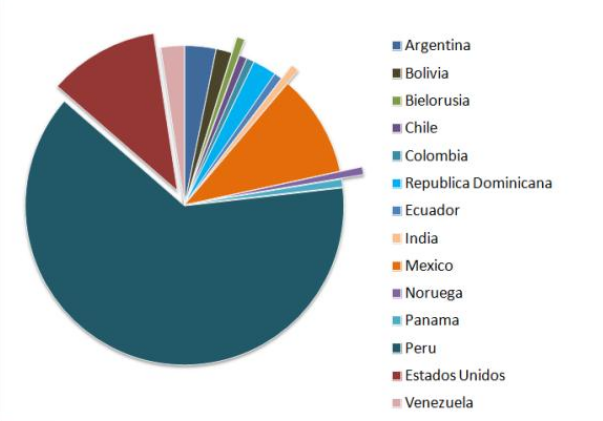
\includegraphics[height=0.8\textheight]{img/estadistica.png}
       \end{center}
    \end{figure}
  
\end{slide}


%



\section{Como realizar un analisis}	

\begin{slide}
  \begin{enumerate}
  \item Reconocimiento -- Tecnologia\pause
  \item Analisis\pause
  \item Experimentacion\pause
  \item Conclusion
  \end{enumerate}
\end{slide}

%%
\section{Como realizar un analisis II}	

\begin{slide}
  Las etapas que se pueden seguir son:
  \begin{itemize}
  \item Recoleccion
  \item Analisis

    \begin{figure}[h]
      \begin{center}
        
\includegraphics[height=0.3\textheight]{img/malwares1.jpg}
      \end{center}
    \end{figure}

  \item Conclusion
  \end{itemize}
\end{slide}

%%

\subsection{Recoleccion}
\begin{slide}  
    \begin{figure}
      \begin{center}
        
\includegraphics[height=0.3\textheight]{img/youtubeface.png} \\
 
\includegraphics[height=0.5\textheight]{img/face.png}
      \end{center}
    \end{figure}
\end{slide}

%%

\begin{slide}
    \begin{figure}
      \begin{center}
        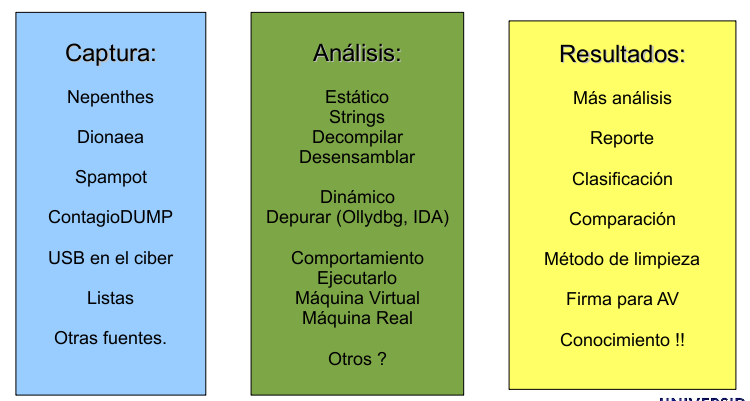
\includegraphics[height=0.8\textheight]{img/arq.png}
      \end{center}
    \end{figure}

\end{slide}

%%

%%

\section{Un analisis REAL}

%%

\begin{slide}
  \begin{itemize}
  \item Creación de un ambiente controlado\pause
  \item Análisis Estático\pause
  \item Análisis Dinamico\pause
  \end{itemize}
\end{slide}

%%

\subsection{Distribuciones}

%%

\begin{slide}

  \begin{block}{REMnux}
    REMnux es la distribución de GNU/Linux basada en Ubuntu de Lenny Zeltser para el análisis e Ingeniería Inversa del Malware (Reverse-Engineering Malware – REM).
  \end{block}

  \begin{block}{Bugtraq y MOBISEC}
    Bugtraq distribución española la cual tiene una sección para el analisis de Malware.\\
    Mobisec distribución orientada al analisis de malware para dispositivos Android.
  \end{block}

\end{slide}

%%

\subsection{Lo que hacemos hoy... }

%%





\begin{slide}

  \begin{exampleblock}{}
    LOS ACTOS PRESENTES DERIVAN LA SITUACION FUTURA.
  \end{exampleblock}}

  \begin{exampleblock}{}
   SOMOS JOVENES Y TENEMOS QUE APRENDER A TENER UNA MEDIDA A NUESTRAS TRAVESURAS, LA INQUIETUD DEBEMOS DE SABER CANALIZAR Y CONTROLARLA.
  \end{exampleblock}}

\end{slide}

%%


%%%%%%%%%%%%%%%%%%%%%%%%%%%%%%%%%%%%%%%%%%%%%%%%%%%%%%%%%%%%%%%%%%%%%%
%%%%%%%%%%%%%%%%%%%%%%%%%%%%%%%%% FIN %%%%%%%%%%%%%%%%%%%%%%%%%%%%%%%%
%%%%%%%%%%%%%%%%%%%%%%%%%%%%%%%%%%%%%%%%%%%%%%%%%%%%%%%%%%%%%%%%%%%%%%

\begin{blankslide}
  \vspace{1cm}
  \begin{center}
    {\Large Gracias por su atención}
  \end{center}
  \vspace{1cm}
  \begin{flushright}
    {\bf \autor}\\
    {\tt \email}\\[0.5cm]
    %% Por favor, respeta esta referencia al autor de la plantilla
    {\scriptsize Presentación compuesta con \LaTeX\ }
  \end{flushright}
\end{blankslide}

\end{document}
